\documentclass{article}

% required package for inserting figures
\usepackage{graphicx}

\setlength{\parindent}{0pt}

\begin{document}

\section{$\pi$ attenuator}
\begin{figure}[ht]
    \centering
    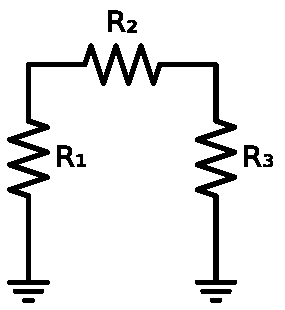
\includegraphics[width=0.3\linewidth]{pi_attenuator_fig.pdf}
    \caption{$\pi$-attenuator}
    \label{fig:pi_attenuator}
\end{figure}

The three constraints for the attenuator,
\begin{enumerate}
    \item \(R_1 = R_3\)
    \item \(S_{11} = 0\), or \(Z_{in} = R_0\)
    \item \(S_{21} = A\)
\end{enumerate}

Starting with the second constraint, when looking into the left side of the network, and assuming
the right side is terminated in \(R_0 = 50\Omega\), \(Z_{in}\) is,

\[Z_{in} = (R_3 || R_0 + R_2) || R_1\]
\[Z_{in} = {\Big({R_3 R_0 \over R_3 + R_0} + R_2\Big) R_1 \over \Big({R_3 R_0 \over R_3 + R_0} + R_2\Big) + R_1} \]
\[Z_{in} = {\Big({R_3 R_0} + R_2 (R_3 + R_0)\Big) R_1 \over \Big({R_3 R_0} + R_2 (R_3 + R_0)\Big) + R_1 (R_3 + R_0)} \]

Using \(R_1 = R_3\), and the constraint that \(Z_{in} = R_0\),
\[R_0 = {\Big({R_1 R_0} + R_2 (R_1 + R_0)\Big) R_1 \over \Big({R_1 R_0} + R_2 (R_1 + R_0)\Big) + R_1 (R_1 + R_0)} \]

Solve for \(R_2\),
\[R_0 \Big(\Big({R_1 R_0} + R_2 (R_1 + R_0)\Big) + R_1 (R_1 + R_0)\Big) = {\Big({R_1 R_0} + R_2 (R_1 + R_0)\Big) R_1 } \]
\[R_0  R_2 (R_1 + R_0) - R_1 R_2 (R_1 + R_0)=  {{R_1^2 R_0} } - R_1 R_0^2 - R_0 R_1 (R_1 + R_0)\]
\[ R_2 \Big(R_0 (R_1 + R_0) - R_1 (R_1 + R_0) \Big)=  {{R_1^2 R_0} } - R_1 R_0^2 - R_0 R_1 (R_1 + R_0)\]
\[ R_2 =  {{R_1^2 R_0}  - R_1 R_0^2 - R_0 R_1 (R_1 + R_0) \over R_0 (R_1 + R_0) - R_1 (R_1 + R_0)}\]

\[ R_2 =  { 2R_1 R_0^2 \over R_1^2  - R_0^2 } \]

The third constraint requires the voltage transfer function to be equal to the desired voltage loss, A. 

\[S_{21} = {V_2^- \over V_1^+} \Bigg|_{V_2^+ =0} = A\]

Since the input impedance is matched, \(V_1^- = 0\), and because the s-parameter definition requires that \(V_2^+ =0\),

\[A = {V_2 \over V_1} \]

If a voltage \(V_1\) is applied at port 1, the voltage at port 2 is,

\[V_2 = V_1 {R_3 || R_0 \over R_2 + R_3 || R_0} \]

\[{V_2 \over V_1}=  {R_3 || R_0 \over R_2 + R_3 || R_0} \]
\[{V_2 \over V_1}=  {{R_3 R_0 \over R_3 + R_0} \over R_2 + {R_3 R_0 \over R_3 + R_0} } \]
\[{V_2 \over V_1}=  {{R_3 R_0} \over R_2 (R_3 + R_0)+ {R_3 R_0} } \]

Again using \(R_1 = R_3\),

\[A = {V_2 \over V_1}=  {{R_1 R_0} \over R_2 (R_1 + R_0)+ {R_1 R_0} } \]

Solve for \(R_2\),
\[AR_2 (R_1 + R_0)+ A{R_1 R_0} = {{R_1 R_0}} \]
\[R_2 = {{R_1 R_0} - A{R_1 R_0} \over A(R_1 + R_0)}\]
\[R_2 = {{R_1 R_0}(1 - A) \over A(R_1 + R_0)}\]

We have two unknowns, \(R_1\) and \(R_2\), with two equations,

\[ R_2 =  { 2R_1 R_0^2 \over R_1^2  - R_0^2 } \]
\[R_2 = {{R_1 R_0}(1 - A) \over A(R_1 + R_0)}\]

Equating,
\[ {{R_1 R_0}(1 - A) \over A(R_1 + R_0)} =  { 2R_1 R_0^2 \over R_1^2  - R_0^2 } \]

Solving for \(R_1\),
\[ {{R_1 R_0}(1 - A) (R_1^2  - R_0^2 ) } =  { 2R_1 R_0^2 A(R_1 + R_0)} \]
\[ {(1 - A) (R_1^2  - R_0^2 ) } =  { 2R_0 A(R_1 + R_0)} \]
\[ {(1 - A) (R_1^2)} -2R_0 A(R_1) =  { 2R_0^2 A } + R_0^2(1 - A) \]
\[ {(1 - A) (R_1^2)} -2R_0 A(R_1) - R_0^2(A + 1) = 0\]
\[ {(1 - A) (R_1^2)} -2R_0 A(R_1) + R_0^2(1 - A) = 0\]


Using the quadratic formula to solve for \(R_1\),
\[R_1 = {{ 2 R_0 A} \pm \sqrt{  4A^2R_0^2 - 4 R_0^2 (1 - A) (A + 1)} \over 2(1 - A)} \]
\[R_1 = {{ R_0 A} \pm R_0 \sqrt{  A^2 - (A^2 + 1)} \over (1 - A)} \]
\[R_1 = R_0{{  A} \pm  1 \over 1 - A} \]

A is less than 1 (since attenuator is passive), so the denominator is always positive. For \(R_1\) to be non-negative, we must take the \(A +1\)
solution,
\[R_1 = R_0{ A +  1 \over 1 - A} \]

Using this in the equation for \(R_2\),
\[R_2 = {{R_1 R_0}(1 - A) \over A(R_1 + R_0)}\]
\[R_2 = {R_0{{ A +  1 \over 1 - A}  R_0}(1 - A) \over A(R_0{ A +  1 \over 1 - A}  + R_0)}\]
\[R_2 = {R_0 (A + 1)\over A({ A +  1 \over 1 - A}  + 1)}\]
\[R_2 = R_0{ (A + 1)(1 - A)\over A({ A +  1 }  + (1 - A))}\]
\[R_2 = {R_0 } { 1 - A^2 \over  2A}\]

% \[R_1 = {-{ 2R_0} \pm 2\sqrt{  R_0^2 - (1 - L^2)} \over 2(1 - L)} \]
% \[R_1 = {-{ R_0} \pm \sqrt{  R_0^2 + L^2 -1 } \over 1 - L} \]


% Use the equation for \(R_2\) in the equation for \(A\), and using \(L = {1 \over A}\)

% \[-{ 2R_1 R_0^2 \over R_0^2 - R_1^2 } (R_1 + R_0)+ {R_1 R_0} = {{R_1 R_0} L} \]

% \[-{ 2R_1 R_0^2 } (R_1 + R_0)+ {R_1 R_0}({R_0^2 - R_1^2 }) = {{R_1 R_0} L} (R_0^2 - R_1^2 )\]

% Divide by \(R_1\) and \(R_0\),
% \[-{ 2R_1 R_0} - 2R_0^2 + R_0^2 - R_1^2 = L{R_0^2} - L{R_1^2}\]

% Negate both sides,
% \[{ 2R_1 R_0} + R_0^2 + R_1^2 = -L{R_0^2} + L{R_1^2}\]

% Group like terms,
% \[R_1^2(1 - L)  + R_1({2R_0}) +  R_0^2(1 + L)  = 0\]

% Using the quadratic formula to solve for \(R_1\),
% \[R_1 = {-{ 2 R_0} \pm \sqrt{  4R_0^2 - 4 (1 - L) (1 + L)} \over 2(1 - L)} \]
% \[R_1 = {-{ 2R_0} \pm 2\sqrt{  R_0^2 - (1 - L^2)} \over 2(1 - L)} \]
% \[R_1 = {-{ R_0} \pm \sqrt{  R_0^2 + L^2 -1 } \over 1 - L} \]





\end{document}